\documentclass[11pt]{article}
\usepackage{fullpage}
\usepackage{setspace}
\usepackage{amsmath}
\usepackage{fancyvrb}
\usepackage{enumerate}
\usepackage{listings}
\usepackage{pgfplots}
\usepackage{graphicx}
\usepackage{float}
\usepackage{multirow}
\usepackage[format=hang,labelsep=quad]{caption}
\usepackage{subfig}
\usepackage{array}
\usepackage{multirow}

\renewcommand\thesubfigure{\roman{subfigure}}


\begin{document}
\noindent\large{Math 5364}\\
\large{Data Mining 2}\\
\large{Homework 22}\\
\large{Mary Barker}
\doublespace

\begin{enumerate}
    \item Import the data set BIO120.txt, which contains data for 3146 Biol 120 students, 
    including the following variables: 
    \begin{itemize}
	\item Grade: 1 = A, B, or C, 0 = all other grades.
	\item Rank: Percentile rank represented as a decimal between 0 and 1, w 
              values close to 1 corresponding to higher ranked students. 
	\item Math and Verbal: Math and Verbal SAT scores
	\item Prev: 1 = student has taken Bio120 before, and 0 = student has not
	\item Rdg: Status of student regarding the remedial course Reading 100. 
              possible levels are Never Taken, Concurrently Enrolled, Passed, and Failed. 
	\item Father's and Mother's education levels
	\item Gender
    \end{itemize}

    \item Build the best possible logistic regression model for predicting grade based on 
     the other variables.

	\begin{enumerate}
		\item Divide the data set into two parts for the purpose of cross-validation. 

		\item  Fit a univariate model regressing grade onto each of the other variables. 
	         For the quantitative variables, attempt to determine if higher order terms 
	         are needed using the groupplot function (see LogisticRegressionFunctions.txt 
	         for some helpeful functions). As with linear regression, you can use a 
	         likelihood ratio test to formally test whether these terms are needed 
	         (LRtest function)
	         For the categorical variables, a univariate model can help to determine if 
	         some of the levels can be grouped together to create a variable with fewer 
	         levels. This is essential for the father and mother variables which have 8 
	         levels. It is likely that a stepwise regression will eliminate one of the 
	         parent's education variables, since they are highly correlated and have a 
	         large number of parameters. 

\begin{Verbatim}
basicmodel <- glm(grade~., data = bio.train, family=binomial)
summary(basicmodel)
\end{Verbatim}

		\begin{center}
			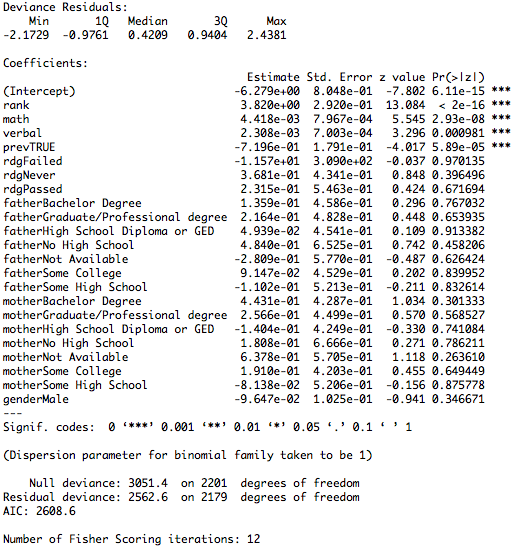
\includegraphics[scale=0.7]{basicmodel_summary}
		\end{center}

		\begin{itemize}

			\item Rank
\begin{Verbatim}
rank.model1 = glm(grade~rank, data=bio.train, family=binomial)
summary(rank.model1)
\end{Verbatim}
		\begin{center}
			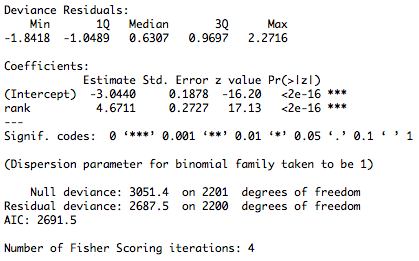
\includegraphics[scale=0.7]{rank_model1}
		\end{center}
\begin{Verbatim}
LRtest(rank.model1, basicmodel)
\end{Verbatim}

	The result for the \verb|LR| test was 1.110223e-16.

			In order to check whether high order terms are necessary, 
			first we will generate logit plots to view the curvature. 

			\begin{figure}[H]
				\caption{Logit plot for rank and grade with degree 1}
				\begin{center}
					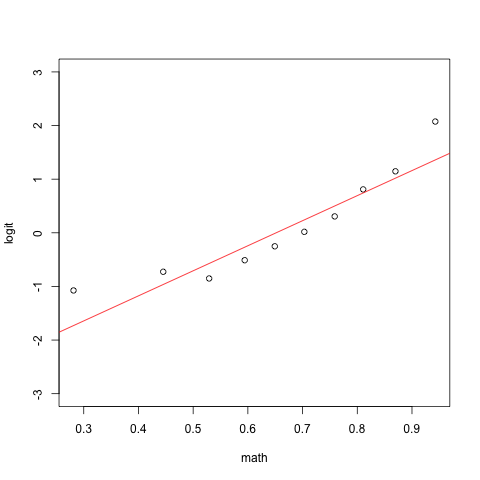
\includegraphics[scale=0.25]{grade_rank_logit}
				\end{center}
			\end{figure}

			\begin{figure}[H]
				\caption{Logit plot for rank and grade with degree 2}
				\begin{center}
					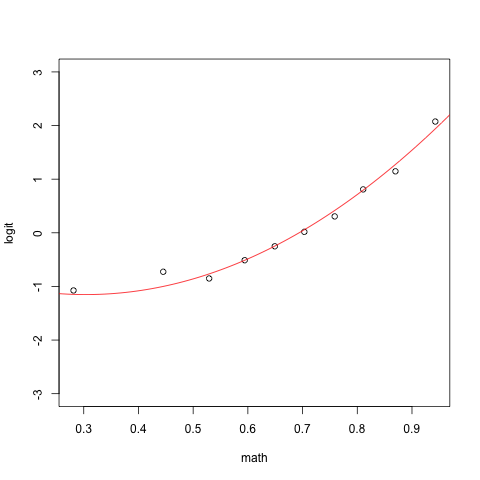
\includegraphics[scale=0.25]{grade_rank_logit_deg2}
				\end{center}
			\end{figure}
\begin{Verbatim}
rank.model2 = glm(grade~rank+I(rank^2), data=bio.train, family=binomial)
summary(rank.model2)
\end{Verbatim}
		\begin{center}
			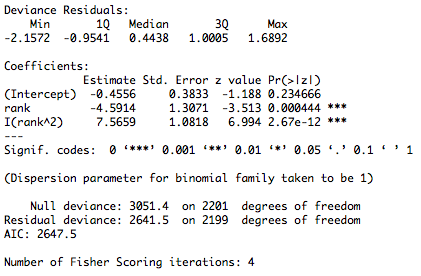
\includegraphics[scale=0.7]{rank_model2}
		\end{center}
\begin{Verbatim}
LRtest(rank.model2, basicmodel)
\end{Verbatim}

	The result for the \verb|LR| test was 6.023138e-09.

\begin{Verbatim}
rank.model3 = glm(grade~rank+I(rank^2)+I(rank^3), data=bio.train, family=binomial)
summary(rank.model3)
\end{Verbatim}
		\begin{center}
			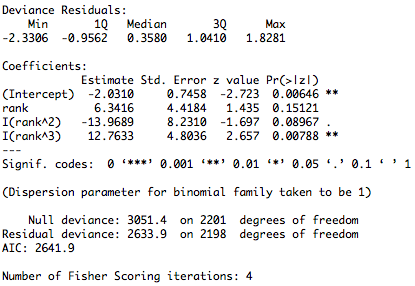
\includegraphics[scale=0.7]{rank_model3}
		\end{center}
\begin{Verbatim}
LRtest(rank.model3, basicmodel)
\end{Verbatim}
	The result for the \verb|LR| test was 5.600436e-08.

\begin{Verbatim}
rank.model4 = glm(grade~rank+I(rank^2)+I(rank^3)+I(rank^4), data=bio.train, family=binomial)
summary(rank.model4)
\end{Verbatim}
		\begin{center}
			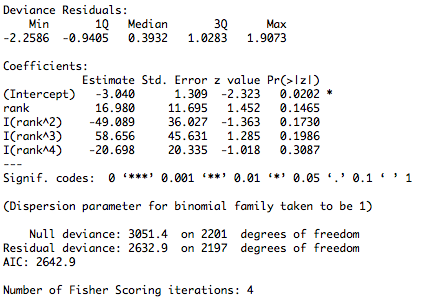
\includegraphics[scale=0.7]{rank_model4}
		\end{center}
\begin{Verbatim}
LRtest(rank.model4, basicmodel)
\end{Verbatim}
	The result for the \verb|LR| test was 4.13323e-08.

		\item Math
\begin{Verbatim}
math.model1 = glm(grade~math, data=bio.train, family=binomial)
summary(math.model1)
\end{Verbatim}
		\begin{center}
			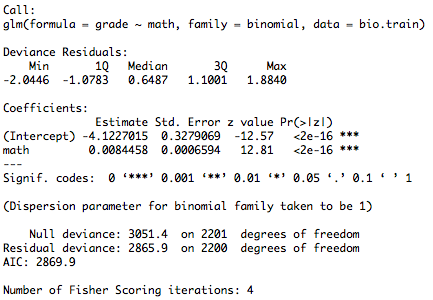
\includegraphics[scale=0.7]{math_model}
		\end{center}
\begin{Verbatim}
LRtest(math.model1, basicmodel)
\end{Verbatim}
	The result for the \verb|LR| test was 0.


			\begin{figure}[H]
				\caption{Logit plot for math and grade with degree 1}
				\begin{center}
					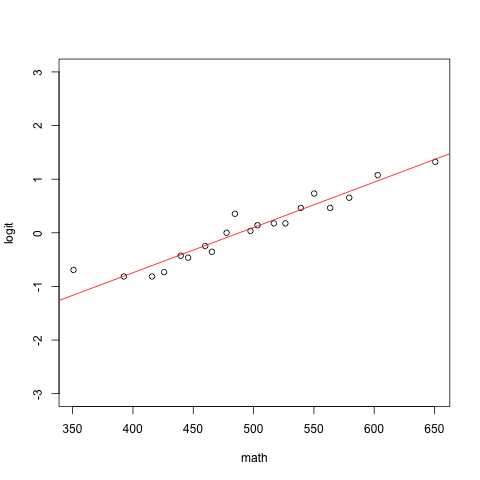
\includegraphics[scale=0.25]{grade_math_logit}
				\end{center}
			\end{figure}
          doesn't look like HOT will help. 

		\item Verbal
\begin{Verbatim}
verbal.model1 = glm(grade~verbal, data=bio.train, family=binomial)
summary(verbal.model1)
\end{Verbatim}
		\begin{center}
			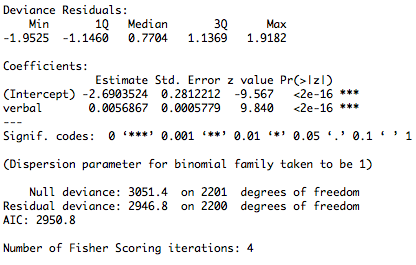
\includegraphics[scale=0.7]{verbal_model}
		\end{center}
\begin{Verbatim}
LRtest(verbal.model1, basicmodel)
\end{Verbatim}
	The result for the \verb|LR| test was 0.


			\begin{figure}[H]
				\caption{Logit plot for verbal and grade with degree 1}
				\begin{center}
					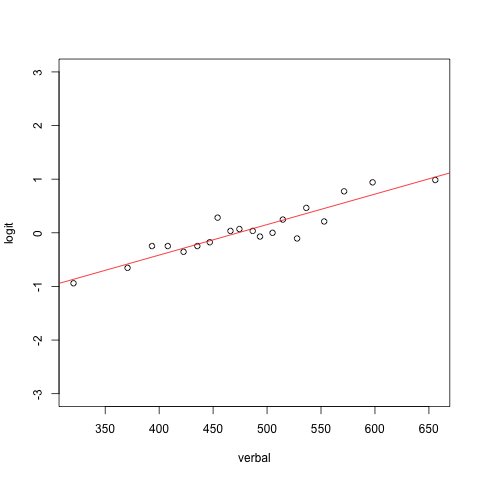
\includegraphics[scale=0.25]{grade_verbal_logit}
				\end{center}
			\end{figure}
          doesn't look like HOT will help. 

		\item Prev
\begin{Verbatim}
prevmodel = glm(grade~rank+math+verbal+rdg+father+mother+gender, data=bio.train, family=binomial)
LRtest(prevmodel, basicmodel)
\end{Verbatim}
	The result for the \verb|LR| test was 3.690684e-05.

		\item Gender 
\begin{Verbatim}
gendermodel = glm(grade~rank+math+verbal+prev+rdg+father+mother, data=bio.train, family=binomial)
LRtest(gendermodel, basicmodel)
\end{Verbatim}
	The result for the \verb|LR| test was 0.346872.

		\item rdg
\begin{Verbatim}
rdgmodel = glm(grade~rank+math+verbal+prev+father+mother+gender, data=bio.train, family=binomial)
LRtest(rdgmodel, basicmodel)
\end{Verbatim}
	The result for the \verb|LR| test was 0.5859034.

		\item Father
\begin{Verbatim}
fathermodel = glm(grade~rank+math+verbal+prev+rdg+mother+gender, data=bio.train, family=binomial)
LRtest(fathermodel, basicmodel)
\end{Verbatim}
	The result for the \verb|LR| test was 0.8947546.

\begin{Verbatim}
father.recode = c('HighSchool/SomeCollege', 
                  'Bachelor/Grad', 
                  'Bachelor/Grad', 
                  'HighSchool/SomeCollege', 
                  'NoHighSchool/SomeHighSchool', 
                  'NA', 
                  'HighSchool/SomeCollege', 
                  'NoHighSchool/SomeHighSchool')

new.father = father.recode[bio$father] %$
new.father.model = glm(grade~rank+math+verbal+prev+rdg+mother+gender+new.father[train], 
                       data=bio.train, family=binomial)
summary(new.father.model)
\end{Verbatim}
		\begin{center}
			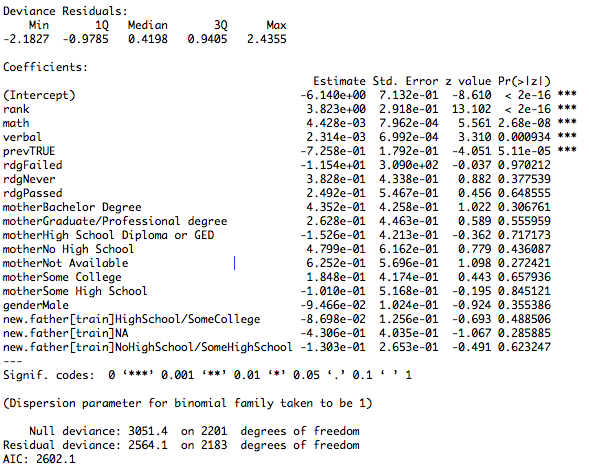
\includegraphics[scale=0.7]{newfathersummary}
		\end{center}

\begin{Verbatim}
LRtest(new.father.model, basicmodel)
\end{Verbatim}
	The result for the \verb|LR| test was 0.8278164.

		\item Mother 
\begin{Verbatim}
mothermodel = glm(grade~rank+math+verbal+prev+rdg+father+gender, data=bio.train, family=binomial)
LRtest(mothermodel, basicmodel)
\end{Verbatim}
	The result for the \verb|LR| test was 0.02942975.

\begin{Verbatim}
mother.recode = c('HighSchool/SomeCollege', 
                  'Bachelor/Grad', 
                  'Bachelor/Grad', 
                  'HighSchool/SomeCollege', 
                  'NoHighSchool/SomeHighSchool', 
                  'NA', 
                  'HighSchool/SomeCollege', 
                  'NoHighSchool/SomeHighSchool')

new.mother = mother.recode[bio$mother] %$
new.mother.model = glm(grade~rank+math+verbal+prev+rdg+father+gender+new.mother[train], 
                       data=bio.train, family=binomial)
summary(new.mother.model)
LRtest(new.mother.model, basicmodel)
\end{Verbatim}
	The result for the \verb|LR| test was 0.1521139

\begin{Verbatim}
mother.recode = c('NA', 
                  'Bachelor/Grad', 
                  'Bachelor/Grad', 
                  'HighSchool/SomeCollege', 
                  'NoHighSchool', 
                  'NA', 
                  'HighSchool/SomeCollege', 
                  'SomeHighSchool')
new.mother = mother.recode[bio$mother] %$
new.mother.model = glm(grade~rank+math+verbal+prev+rdg+father+gender+new.mother[train], 
                       data=bio.train, family=binomial)
summary(new.mother.model)
LRtest(new.mother.model, basicmodel)
\end{Verbatim}
	The result for the \verb|LR| test was 0.05273772.
	\end{itemize}

	\item Use stepwise and best subsets methods to narrow down the list of predictor 
	         variables. Given the small number of predictor variables, you can also adopt 
	         a manual selection approach to select the variables or to modify the results 
	         of the stepwise/best subsets procedures.

\begin{Verbatim}
model = glm(grade~rank+math+verbal+prev+rdg+father+new.mother[train]+gender, 
             data=bio.train, family=binomial)
step.model=step(model)

X = model.matrix(model)
X = X[,2:ncol(X)]
y = bio.train$grade %$
Xy = data.frame(X,y)

best.model = bestglm(Xy, family=binomial)
summary(best.model$BestModel) %$
\end{Verbatim}
		\begin{center}
			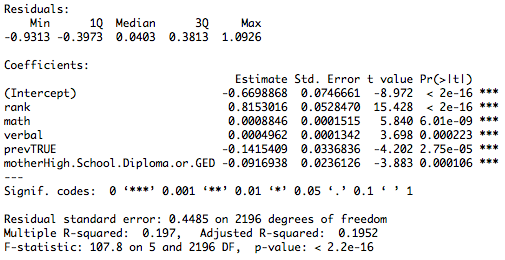
\includegraphics[scale=0.7]{best_model_summary}
		\end{center}
          Conclusion: keep rank, math, verbal, prev, new.mother


	\item Fit a tentative final model. The quantitative variables should be checked again
          for functional form and categorical variables should be checked for groupings. 
          You can also consider adding interaction terms. 

\begin{Verbatim}
tentative.final = glm(grade~rank+I(rank^2)+I(rank^3)+I(rank^4)+math+verbal+prev+mother, 
                      data=new.bio[train,], family=binomial)
summary(tentative.final)
\end{Verbatim}
		\begin{center}
			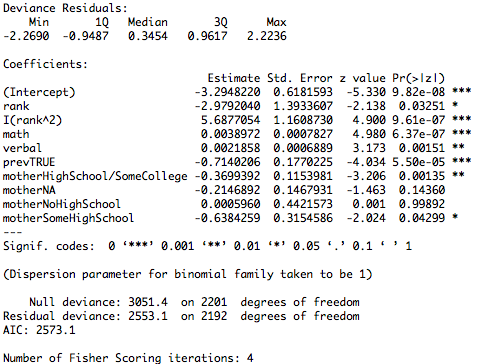
\includegraphics[scale=0.7]{tentative_summary}
		\end{center}

	\item Assess the performance of the model by determining its classification accuracy 
         using a cutoff probability of 0.5 and finding the area under the ROC curve. 
         Each of these metrics can be calculated from the training sample using 
         leave-one-out or delete-d cross-validation, and they can be calculated using 
         the validation sample. 

\begin{Verbatim}
results = predict(tentative.final, new.bio[-train,], type='response')
predicted.grade = (results >= 0.5) * 1
table(predicted.grade)
myacc <- confmatrix(bio$grade[-train], predicted.grade) %$
\end{Verbatim}
	The result for the \verb|LR| test was 0.7256356.


		\begin{center}
			
\includegraphics[scale=0.25]{roc_curve}
		\end{center}

	\item Finally, assess the fit of the final model using the Hosmer-Lemeshow goodness-
         of-fit test.

\begin{Verbatim}
Pihat = predict(tentative.final, type='response')
HLgof.test(fit=Pihat, obs=bio.train$grade) %$
\end{Verbatim}
		\begin{center}
			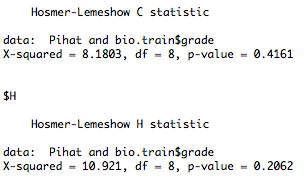
\includegraphics[scale=0.7]{hl_gof_summary}
		\end{center}

	\end{enumerate}
\end{enumerate}

\pagebreak
\lstinputlisting[language=R, basicstyle=\ttfamily\scriptsize]{hw22.R}
\end{document}
